%% ROOT FILE

\documentclass[chap]{thesis}

% prevent orphan lines
\usepackage[all]{nowidow}

%% Some Useful Packages
\usepackage{url} % pretty urls
\usepackage{hyperref} % links within the document
\usepackage{graphicx} % insert graphical files

%% ADD OTHER PACKAGES HERE

% ------------------------
% Attribution of previously published work
%
% Use the after title and before the first sentence of the chapter
% Example: \blfootnote{This work perviously appeared as: \bibentry{mypaper2015}
\makeatletter
\def\blfootnote{\xdef\@thefnmark{}\@footnotetext}
\makeatother
\usepackage{bibentry}
\nobibliography*

% If you have an attribution before your first in-text citation,
% you should use \nobibentry to ensure in-text citations start at [1]
% Example: \blfootnote{This work perviously appeared as: \nobibentry{mypaper2015}
\newcommand{\ignore}[1]{}
\newcommand{\nobibentry}[1]{{\let\nocite\ignore\bibentry{#1}}}
% ------------------------

\begin{document}

%%%%%%%%%%%%%%%%%%%%%%%%%%%%%%%%%%%%%%%%%%%%%%%%%%%%%%%%%%%%%%%%%%%
%  This file produces the title page, copyright page (if requested)
%  and the Table of Contents, List of Figures and List of Tables.
%%%%%%%%%%%%%%%%%%%%%%%%%%%%%%%%%%%%%%%%%%%%%%%%%%%%%%%%%%%%%%%%%%%

% Supply information for use on title page:
%
\thesistitle{\bf My Super Thesis Template}
\author{Elsa Gonsiorowski}
\degree{Doctor of Philosophy}
\department{Computer Science}

\signaturelines{4}     %max number of signature lines is 7
\thadviser{Christopher D. Carothers}
\memberchair{Mark Shephard}
\memberone{Barbara Cutler}
\membertwo{Tong Zhang}

\submitdate{December 2015\\(For Graduation May 2016)}
%\copyrightyear{2015}   % if omitted, current year is used.

% Print titlepage and other prefatory material:
%
\titlepage
%\copyrightpage         % optional
\tableofcontents
\listoftables          % required if there are tables
\listoffigures         % required if there are figures


%%%%%%%%%%%%%%%%%%%%%%%%%%%%%%%%%%%%%%%%%%%%%%%%%%%%%%%%%%%%%%%%%%%
%                                                                 %
%                         ACKNOWLEDGEMENT                         %
%                                                                 %
%%%%%%%%%%%%%%%%%%%%%%%%%%%%%%%%%%%%%%%%%%%%%%%%%%%%%%%%%%%%%%%%%%%

\specialhead{ACKNOWLEDGMENT}

Just remember one thing:

{\it ``Every academic has that one study they wish they would have prepared better for. The one they regret. The one they call a dissertation.''}
--- Nathan Hall

%%%%%%%%%%%%%%%%%%%%%%%%%%%%%%%%%%%%%%%%%%%%%%%%%%%%%%%%%%%%%%%%%%%
%                                                                 %
%                            ABSTRACT                             %
%                                                                 %
%%%%%%%%%%%%%%%%%%%%%%%%%%%%%%%%%%%%%%%%%%%%%%%%%%%%%%%%%%%%%%%%%%%

\specialhead{ABSTRACT}

Large LaTeX documents are sufficiently hard to set up.
This thesis repository is organized and ready for you to start writing.

Get ready to graduate!

\chapter{Introduction and Contributions}
\label{chapt:intro}

\blfootnote{Portions of this chapter previously appeared as: \nobibentry{me:mascots:2012}}

An introduction to the thesis.
Despite the footnote, here is my first citation~\cite{jefferson-tw}.

I think it is tacky to have a section without an intro text.

\section{Circuit Design}

I have a pretty image, see Figure~\ref{fig:design-process}.

\begin{figure*}[ht]
\centering
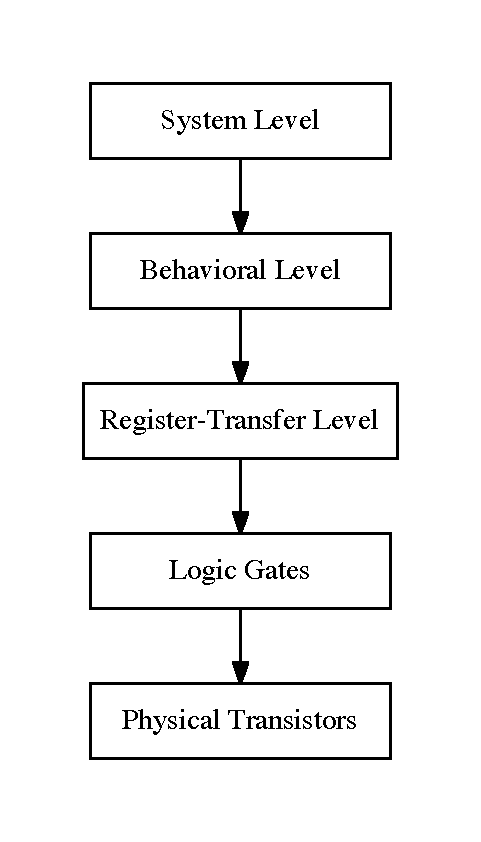
\includegraphics[width=0.4\textwidth]{figs/cdp.pdf}
\caption [Circuit Design Process Levels of Abstraction] {
	Levels of abstraction within the circuit design process.
	Automatic tools perform synthesis on a given design to generate the design at the next (lower) level.
	This design is then validated through one or more tests.
}
\label{fig:design-process}
\end{figure*}




\section{Contributions}

You thesis committee is very smart.
Prove that you are smart by clearly stating what your contributions are.

\subsection{Contribution 1: Publication 1}

I did a thing and published the work.

\subsection{Contribution 2: Other thing}

Some other thing I did.

\subsection{Contribution 3: Final Thing}

Also this.

\section{Thesis Organization}

This document begins by presenting the necessary background (include domain specific terminology and related works) for understanding my contributions (Chapter~\ref{chapt:bg}).
I then present a working proof-of-concept experiment (Chapter~\ref{chapt:pub1}).
The challenges faced in this proof-of-concept experiment lead to my research on three distinct problems:
\begin{itemize}
  \item Thing A (Chapter~\ref{chapt:a});
  \item Thing B (Chapter~\ref{chapt:b});
  \item Thing C (Chapter~\ref{chapt:c});
\end{itemize}
Finally, I present my research contributions and discuss the conclusions drawn from these experiments (Chapter~\ref{chapt:conc}).

\chapter{Background and Related Work}
\label{chapt:bg}

\blfootnote{Portions of this chapter previously appeared as: \bibentry{me:mascots:2012}}

This thesis describes a software-base workflow for transforming a domain specific design into PDES model.
To understand the nuances of this problem, this chapter provides an overview of parallel simulation and the circuit modeling domain.
It also presents related work in this area.

% What is PDES
\section{Parallel Simulation}

Computer simulations model real world behavior in order to understand a complex system over time.
Within discrete-event simulations the state of the modeled system can only be modified through a sequence of time-stamped events~\cite{book:simulation}.
Thus these simulations are constructed through two entities:
\begin{itemize}
	\item Events:\\
		  Each event occurs at a particular instance in time and contains a specific piece of information.
		  An event will directly affect only one logical process, but a series of events can be said to be causally linked.
	\item \textit{Logical Processes} (LPs):\\
		  These entities encapsulate the particular state of a portion of the modeled system.
		  LPs are directly affected by events, and can cause change to other parts of the system by ``sending'' or ``scheduling'' events in the future.
\end{itemize}


When a simulation engine exists within a parallel or distributed environment it falls in the research area of \textit{Parallel Discrete-Event Simulation} (PDES).
The primary challenge that a legitimate PDES engine must address is that of unique event serializability~\cite{Fujimoto:2000fk}.
That is, the ordering of events within a simulation must be deterministic across any underlying configuration of execution hardware (whether executed in a single processor environment or on any number of parallel processor configurations).
There are two approaches used by parallel simulation engines to achieve the strict and reproducible order of events: conservative and optimistic synchronization~\cite{Fujimoto:2000fk}.
These methods tackle how order the processing (or execution) of events both on global and local scale.
Note that within a parallel system, some segment of the whole or ``global'' problem is considered ``local'' to a single \textit{processing element} (PE, also known as a processor or core).

\subsection{Conservative Synchronization}

Conservative synchronization within a parallel simulation engine ensures that there is both local and global in-order execution of events.
That is, through a conservative synchronization algorithm, no LP is allowed to process an event unless it can be proven that all earlier events which affect the given LP have already been processed.

The seminal approach for processing discrete-events in parallel is the Null Message algorithm developed by Chandy and Misra~\cite{chandy-1981,chandy-misra-1979} and Bryant~\cite{bryant-1977} (also known as the CMB algorithm).
This algorithm synchronizes LPs by \textit{null messages}, messages which contain no information other than a timestamp.
For every event an LP processes, it sends a null message with the that event's timestamp to every other LP in the simulation.
This serves as a guarantee that all future events from the originating LP will have a timestamp greater than or equal to the timestamp contained in the null message.
This algorithm is guaranteed to avoid deadlock when there is a required, non-zero timestamp increment.
That is, upon processing an event at time $t$, the given LP can only schedule events at time $t+\epsilon$.

An alternative approach, and one that more common in modern PDES engines, is the YAWNS algorithm (from ``Yet Another Windowing Network Simulator'')~\cite{yawns}.
This conservative algorithm uses global synchronization coupled with a local processing window (called the \textit{global lookahead} window).
The global lookahead is used to determine the minimum allowable timestamp increment for events.
That is, upon processing an event at time $t$, the given LP can only schedule events at a time greater than $t+global\ lookahead$.
The simulation progresses through the following algorithm:
\begin{enumerate}
	\item Global synchronization:\\
		  All LPs calculate the smallest timestamp on any unprocessed event in the system (called \textit{lower bound timestamp} or LBTS).
		  This is completed through a parallel barrier and reduction algorithm.
	\item Local Processing:\\
		  LPs process all events whose timestamps are less than $LBTS + global\ lookahead$.
		  The constraint of the global minimum timestamp increment creates the guarantee that no event can be scheduled within the current $LBTS + global\ lookahead$ window.
		  When all local events have been processed, the global synchronization step is repeated and time progresses forward to the next LBTS.
\end{enumerate}

The relationship between lookahead window size and the average length of event delay within in a system greatly impacts the speedup that can be achieved by a conservative simulation.
If the lookahead window is relatively small in comparison to the average event delay, there will be negative impact on conservative performance.
This is due to the fact that global synchronization must happen more frequently as the simulation progresses.
If all event delays are of a uniform size, then the lookahead window can be quite large and conservative simulation can perform increasingly well.

\subsection{Optimistic Synchronization}

Within optimistically synchronized parallel simulations there is no guarantee of global in-order execution of events.
This means that an LP may process a sequence of events out of serial order.
The most prevalent algorithm in this area is Time Warp~\cite{jefferson-tw}.
This method keeps track of inter-event causality.
As such, when an out-of-order event is detected, the system is able to recover.

System recovery occurs at an LP level.
One method of LP recovery is called \textit{reverse computation}~\cite{carothers-rc}.
This method uses a function to ``un-process'' a given event.
This allows LPs to \textit{rollback} or \textit{reverse} the effects of a series of events and begin forward event processing with a more correct ordering.
Currently, this function must be provided by the model.

Like conservative synchronization approaches, Time Warp systems do maintain some level of global synchronization.
This is called \textit{global virtual time} (GVT) and it is the the lowest timestamp of an existing unprocessed event.
GVT is used to ensure that there is forward progress of global simulation time and thus requires timestamp increments to be non-negative.

When an LP detects out-of-order event, the event is said to cause the LP to {\it rollback}.
This rollback may require that certain messages be canceled.
This cancellation process is done through {\it anti-messages}.
Within Time Warp systems there are two categories of rollbacks~\cite{Fujimoto:2000fk}:
\begin{itemize}
\item {\bf Primary Rollback}\\
  A rollback triggered by receiving a late message.
  For an LP at time $t$, a primary rollback occurs when it receives an event at a time less than $t$.
  This may cause some anti-messages to be sent.
\item {\bf Secondary Rollback}\\
  A rollback triggered by an anti-message corresponding to a message which has already processed by an LP.
\end{itemize}

Alternative methods of system recovery, such as event reconstruction, have been used for circuit simulation before, reverse computation \cite{carothers-rc} is most effective for this work due to small message size.

\section{Circuit Design Process and Simulation}

The circuit design for modern processors is a complex activity.
The design process involves several levels of abstraction and uses simulation for verification.
As a circuit design evolves, the level of abstraction decreases (see Figure~\ref{fig:design-process}).
When a circuit design is finally realized at the logic gate level, the size of the problem to be simulated increases greatly.
Traditionally, this digital logic simulation step has been a bottle neck in the design process.

\section{Related Work}

Workflows and automatic model generation is not a new area of study.
The idea of predefining a conceptual (or generic) model shows up in many fields where simulation is an important part of a larger workflow.

\chapter{Previously Published Work}
\label{chapt:pub1}

\blfootnote{This chapter previously appeared as: \bibentry{me:mascots:2012}}

%I think it is tacky to have a section without an intro text.

\section{Circuit Design}

I have a pretty image, see Figure~\ref{fig:design-process}.

\begin{figure*}[ht]
\centering
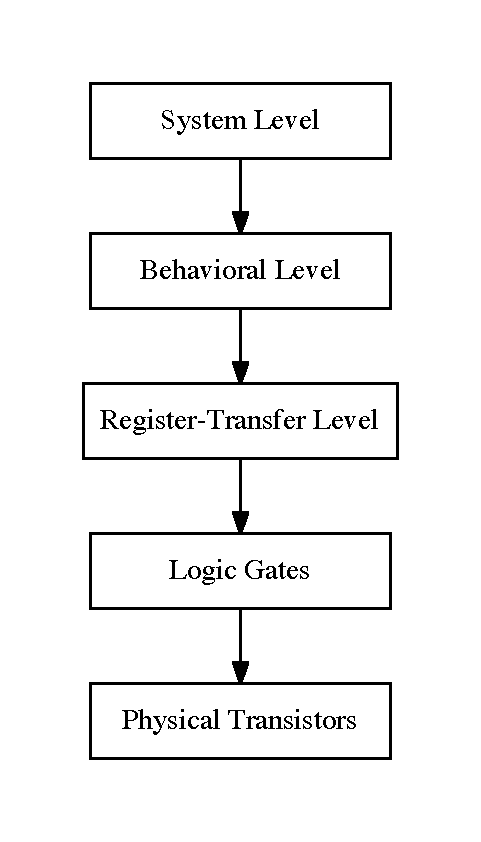
\includegraphics[width=0.4\textwidth]{figs/cdp.pdf}
\caption [Circuit Design Process Levels of Abstraction] {
	Levels of abstraction within the circuit design process.
	Automatic tools perform synthesis on a given design to generate the design at the next (lower) level.
	This design is then validated through one or more tests.
}
\label{fig:design-process}
\end{figure*}



I need some text here in order to be consistent with the rest of my document.

\section{Experiment}

I have this theory...

\section{A thing}

And in conclusion: a thing was done.

%Same.

\section{Finally}

A conclusion.


\section{Summary}

This chapter describes the task of doing a thing.

\chapter{Conclusions and Discussions}
\label{chapt:conc}

Same.

\section{Finally}

A conclusion.


\section{Additionally}

I did great things.

%%%%%%%%%%%%%%%%%%%%%%%%%%%%%%%%%%%%%%%%%%%%%%%%%%%%%%%%%%%%%%%%%%%
%                                                                 %
%                           BIBLIOGRAPHY                          %
%                                                                 %
%%%%%%%%%%%%%%%%%%%%%%%%%%%%%%%%%%%%%%%%%%%%%%%%%%%%%%%%%%%%%%%%%%%

%This method produces a numbered bibliography where the numbers
%correspond to the \cite commands in the text. See the LaTeX manual.
%
\specialhead{REFERENCES}
\begin{singlespace}
\bibliographystyle{bibs/IEEEtran} % sorted by citation order
%\bibliographystyle{bibs/IEEEtranS} % sorted by first author
\bibliography{bibs/IEEEabrv,bibs/simulation}
\end{singlespace}

%%%%%%%%%%%%%%%%%%%%%%%%%%%%%%%%%%%%%%%%%%%%%%%%%%%%%%%%%%%%%%%%%%%%
%                                                                 %
%                            APPENDICES                           %
%                                                                 %
%%%%%%%%%%%%%%%%%%%%%%%%%%%%%%%%%%%%%%%%%%%%%%%%%%%%%%%%%%%%%%%%%%%

\appendix    % This command is used only once!
%\addcontentsline{toc}{chapter}{APPENDICES}             %toc entry  or:
\addtocontents{toc}{\parindent0pt\vskip12pt APPENDICES} %toc entry, no page #


\end{document}
